
%文章相关
\usepackage[UTF8, heading = false, scheme = plain]{ctex}    %解决中文字体,不改变排版
\usepackage{geometry}                                       %调整页边距等
\usepackage{indentfirst}                                    %首行缩进
\usepackage[dvipsnames,svgnames]{xcolor}                    %颜色包:\color{}
\usepackage{enumitem}                                       %控制item的前置符号
\usepackage{adjustbox}                                      %控制文字大小和添加底纹


%图片宏包
\usepackage{graphicx}                                       %插入图片:\includegraphics{myimage.png}
\usepackage{float}
\usepackage{caption}
\usepackage{subcaption}

%数学相关
\usepackage{amsmath,amsthm}                                 %amsmath包应该在前
\usepackage{extarrows}                                      %使用长等号A \xlongequal{\quad\quad}B
\usepackage{cases}                                          %\begin{numcases}可以为方程编号
\usepackage{amssymb}                                        %\checkmark 打勾

%实用的内容说明包
\usepackage{hyperref}                                       %超链接插入包:\href{url}{name}
\usepackage{multirow}                                       %插入表格用到的宏包:\begin{tabular}{|c|c|},&分列,\\分行,\hline插入横线(第二个参数是列数)
\usepackage{listings}                                       %插入代码等:\begin{lstlisting}[breaklines=true,backgroundcolor=\color{lightgray},title=]
\usepackage{verbatim}                                       %使用 comment 环境进行注释


%物理包
\usepackage{physics}
\usepackage{xparse}                                         %physics需求的包
\usepackage{mhchem}                                         %输入原子核的表式\ce{^238_92U}

% \eval{}        根据括号内容的大小在右边添加合适的竖线A|          |         \dv[n]{f}{x}          n阶微分算符 derivative
% \abs{}         添加绝对值|A|                                |         \pdv[n]{f}{x}         n阶偏微分算符 partialderivative
% \norm{}        模||A||                                     |          \bra \ket \braket    左、右、内积
% \comm{}{}      对易子[A,B]                                  |          \op{}{}              外积(密度算符) outerproduct
% \anticomm{}{}  反对易子{A,B}                                |          \ev{<力学量>}{<态>}    期望 expectationvalue
% \vb{}          向量加粗字体                                  |          \mel{}{}{}           矩阵元 matrixelement
% \va{}          向量                                        |          \mqty                 生成矩阵,可跟{} () [] || &分列 \\分行 第一个表示外面无框
% \vu{}          单位向量                                     |         \qty                  合适大小的{}、()等,例如 \qty(x)
% \vdot          点乘                                        |
% \cross         叉乘                                        |
% \grad          梯度 gradient                               |
% \div           散度 divergenc                              |
% \curl          旋度                                        |
% \laplacian     拉普拉斯算符                                 |

%文本底纹实现
\usepackage{lipsum}                                         %该宏包是通过 \lipsum 命令生成一段本文,正式使用时不需要引用该宏包
\usepackage[strict]{changepage}                             %提供一个 adjustwidth 环境
\usepackage{framed}                                         %实现方框效果
%\usepackage{newtxtext}                                     %在macos会报错的一个包注释掉不影响使用
\usepackage{tcolorbox}                                      %文本底纹包,放在xcolor包后
                               
% environment derived from framed.sty: see leftbar environment definition
\definecolor{formalshade}{rgb}{0.95,0.95,1}% 文本框颜色
% ------------------******-------------------
% 注意行末需要把空格注释掉,不然画出来的方框会有空白竖线
\newenvironment{formal}{%
\def\FrameCommand{%
\hspace{-1em}%                                              %框的整体缩进
{\color{Green}\vrule width 0.3em}%                          %竖线颜色以及宽度
\colorbox{greenshade}%                                      %底纹颜色
}%
\MakeFramed{\advance\hsize-\width\FrameRestore}%
\noindent\hspace{-2em}%                                     %禁止第一段文本缩进
\begin{adjustwidth}{}{2em}%                                 %控制右边距        
\vspace{1.5em}%                                             %控制上边距
}
{%
\vspace{1.5em}\end{adjustwidth}\endMakeFramed%              %控制底边距
}%

\definecolor{greenshade}{rgb}{0.90,0.99,0.91}               %绿色文本框,竖线颜色设为 Green
\definecolor{redshade}{rgb}{1.00,0.90,0.90}                 %红色文本框,竖线颜色设为 LightCoral
\definecolor{brownshade}{rgb}{0.99,0.97,0.93}               %莫兰迪棕色,竖线颜色设为 BurlyWood


%使用Mathematica进行计算
%\usepackage{latexalpha2}
%/usr/local/texlive/texmf-local/tex/latex/local/latexalpha2
%直接使用wolfram代码
% \wolfram[<format>]{<code>}    \wolframgraphics[<format>]{<code>}{<filename>} 
%具体使用方法查看 latexalpha2.pdf


%预设
\geometry{a4paper,left=5em,right=5em,bottom=5em,top=5em}    %设置为a4paper最好,点击pacakge geometry 查看文档
\setlength{\parindent}{2em}                                 %2em(注意不支持rem)代表每一段的首行缩进两个字符,某一行不缩进时使用 \noindent

\hypersetup{hidelinks,colorlinks=true,
linkcolor=black,urlcolor=blue}                              %对hyperref 包进行预设

\newenvironment{slt}{\proof[\indent \bf 解 ]}{
\renewcommand{\qedsymbol}{}\endproof}                       %提供解环境
\newtheorem{thm}{定理}[section]                              %定义一个新的环境 thm, 命名为定理,以 节 开始编号
\newtheorem*{thm*}{定理}                                     %定义一个新的环境 thm, 命名为定理,无编号
\newtheorem{lemma}{引理}[section]                            %定义新环境 lemma,命名为引理,以 节 开始编号
\newtheorem*{lemma*}{引理}                                   %定义新环境 lemma,命名为引理,无编号
\newtheorem{corollary}{推论}                                 %定义新环境 corollary,命名为推理,有编号
\newtheorem*{corollary*}{推论}                               %定义新环境 corollary*,命名为推理,无编号
\renewcommand{\proofname}{ \qquad \bf 证明}                  %更改proof为中文证明,proof环境默认存在

%一些def
\def\thmindent{\setlength{\parindent}{5em}}                  %\thmindent
\def\pfindent{\setlength{\parindent}{5.5em}}                 %\pfindent
\def\clindent{\setlength{\parindent}{4em}}                   %clindent
\def\sdr{Schr\"{o}dinger}                                    %薛定谔名字
\def\intff{\int_{-\infty}^{+\infty}}                         %积分为(-\infty,+\infty)的积分
\def\ra{\rightarrow}                                         %右键头\ra
\def\lra{\Longrightarrow}                                    %长(双)右键头\lra
\def\lla{\Longleftarrow}                                     %长(双)左键头\lla
\def\llra{\Longleftrightarrow}                               %等价箭头\llra
\def\xlra{\xlongrightarrow{\quad\quad}}                      %超长右箭头
\def\xlla{\xlongleftarrow{\quad\quad}}                       %超长左箭头
\def\xlla{\xlongleftrightarrow{\quad\quad}}                  %超长等价箭头

\def\psii#1{\psi_{#1}}                                       %常用的\psi下标
\def\psiii#1#2{\psi_{#1} (#2)}                               %常用的\psi下标和括号
\def\psiiii#1#2#3{\psi_{#1}^{#2} (#3)}                       %常用的\psi下标、上标和括号
\def\pe#1#2{E_{#1}^{(#2)}}                                   %能量修正{下标}{上标}
\def\pp#1#2{\psi_{#1}^{(#2)}}                                %波函数修正
\def\ua{a_{+}}                                               %升算符
\def\da{a_{-}}                                               %降算符

\def\nuc#1#2#3{\ce{^{#1}_{#2}{#3}}}                          %原子核的表示形式


%其他备注
\begin{comment}
        求和指标上下方添加        \sum\limits_{}^{}
        恒等于                  \equiv
        远大于                  \gg
        远小于                  \ll
        花括号                  \left\{ \right\}   (建议使用\qty)
        弧度                    37^{\circ}


\end{comment}


%作业包(需要的时候再解除注释)
%\usepackage{iidef}
%建议使用自己的slt解环境
\begin{comment}

    package iidef:
        指定学校名      \thecourseinstitute{}      
        指定课程名      \thecoursename{} 
	    指定学期        \theterm{}
        作业名         \hwname{}
        生成作业标题    \courseheader           放在document环境内 不需要再maketile
        名字           \name                   放在document环境内
        自动编号环境    \begin{enumerate}       [label = (\alph*{})] [label = \arabic*{}.]
        题号           \item                   自动编号,\item[]则不带符号
        证明           \begin{proof}           证明环境由amsthm包提供
        求解           \begin{solution}       
        方程           \begin{equation}        
        方程编号        \labe{eq:[number]}      为方程设置编号  
        引用方程        \eqref{eq:[number]}     引用方程
        行内方程        $...$
        
        多行公式        \begin{align} \begin{align*}则不会编号  
                            ... & = ... \\ 
                                & = ...
                       \begin{array}{lcl}      
                            ... & = & ... \\ 
                            ... & = & ...
        
        方程组          $$
                        \begin{cases}
                       ... & \mbox{if} x \mbox{is even} \\ 带假设
                       $$
                       
                       带编号
                       \begin{numcases}{}
                            \label{1}   \\
                            \label{2}   
                       \end{numcases}
        
        文字大小和底纹
                       \vspace{-1em}
                       \begin{adjustbox}{minipage=0.91\linewidth, bgcolor=gray!20, padding=1em}
                       \small % 将字号变小为 small
                        text
                       \end{adjustbox}
                       \vspace{-1em}

        居中            不要使用$$...$$,会对齐失效 使用$...$即可
                        \begin{center}
            
                        \end{center}

        左对齐           
                        \begin{flushleft}
            
                        \end{flushleft}

        双水平图         \begin{minipage}{0.45\textwidth}
                        \includegraphics[width=\textwidth,keepaspectratio]{./pictures/.png}
                        \end{minipage}
                        \hfill
                        \begin{minipage}{0.45\textwidth}
                            \begin{enumerate}[label = (\arabic*)]
                                \item 
                                \item 
                                \item 
                            \end{enumerate}
                        \end{minipage}

    
\end{comment}




\title{量子力学习题集}
\author{马祥芸}

\begin{document}
    \maketitle
    \tableofcontents
    \newpage
    %\thecoursename{量子力学习题集}  %作业包页眉左边
    %\thecourseinstitute{马祥芸}    %作业包页眉右边

    \section{薛定谔方程与一维定态问题}
        \subsection{一维有限势场}
        \begin{thm}\label{thm:1.1}                                                %添加\lable{书签名}进行标记,使用\pageref{书签名}添加标记位置的页码 \ref{书签名}引用定理编号
            势函数具有偶对称$V(x)=V(-x)$,$\psi(x)$和$\psi(-x)$均是波函数的解
            
            \begin{proof}
                
                $$ \frac{d^2}{[d(-x)]^2}=\frac{d^2}{dx^2} $$ 

            \end{proof}
        
        \end{thm}
    

        \begin{thm}\label{thm:1.2}
            \thmindent
            
            设$V(x)=V(-x)$,\textbf{每一个}$\psi(x)$都有确定的宇称(奇偶性)(注意每一个解的宇称可以不相同)
            
            \begin{proof}
                \pfindent
                
                由于定理\ref{thm:1.1},构造 
                   
                    $$ f(x) = \psi(x)+\psi(-x) $$                          % $$行公式不带编号
                    $$ g(x) = \psi(x)-\psi(-x) $$
                
                $f(x)$为偶宇称,$g(x)$为奇宇称,它们均为能量$E$的解       \par  %另起段落保留缩进
                而$\psi(x)$与$\psi(-x)$都可以用$f(x)$和$g(x)$表示    

                $$ \psi(x) = \frac{1}{2} [f(x)+g(x)]  $$
                $$ \psi(-x) = \frac{1}{2} [f(x)-g(x)] $$    

           \end{proof}
           
           \begin{corollary}\label{cl:1}
                \clindent 
                
                设$V(-x) = V(x)$,而且对应于能量本征值E,方程的解无简并,则该能量本征态必有确定的宇称,例如一维 \par
                谐振子,一维对称方势阱
                
                \begin{itemize}
                    \item 若$E$非简并  \quad 本征函数具有确定宇称(两种宇称) 
                        $$ \psi(-x) = \hat{P}\psi(x) = c\psi \quad c=\pm 1 $$ %\hat{}输入算符的帽子
                    \item 若$E$简并 \quad $\psi(x)$和$\psi(-x)$分别为独立的波函数,它们的线性组合是具有宇称的解
                        $$ \psiii{\pm}{x} = \frac{1}{\sqrt{2}}[\psi(x) \pm \psi(-x)] $$
                \end{itemize}
            
           \end{corollary}

        \end{thm}
        \par
        偶宇称涉及到的函数图像如下

        \begin{figure}[H]
            \centering
            \begin{subfigure}{0.48\textwidth}
                    
                \centering
                \wolframgraphics[png]{Plot[y=Tan[x],{x,0,2.5}]}{tanx}
                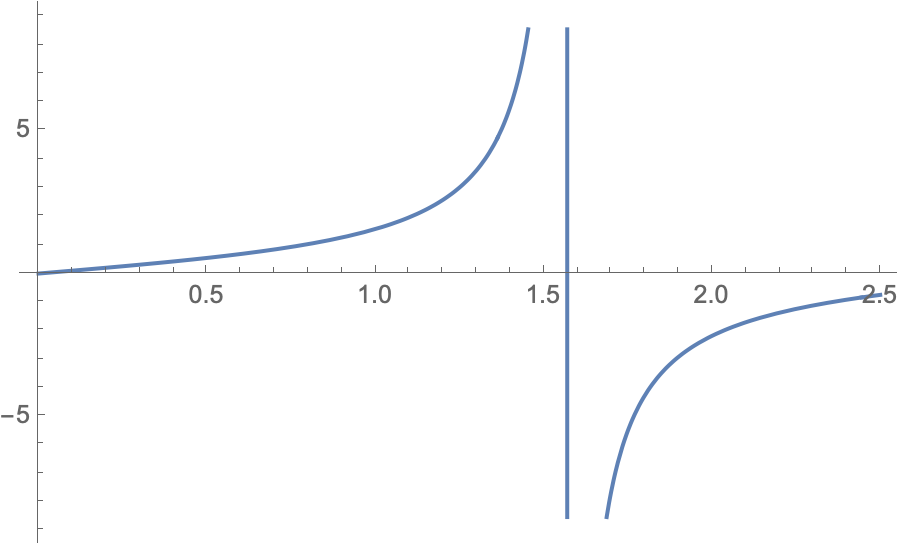
\includegraphics[scale=0.4]{tanx.png}
                \caption{$y=\tan{x}$}
                
            \end{subfigure}
            \begin{subfigure}{0.48\textwidth}
                
                \centering
                \wolframgraphics[png]{Plot[y=x*Tan[x],{x,0,2.5}]}{xtanx}
                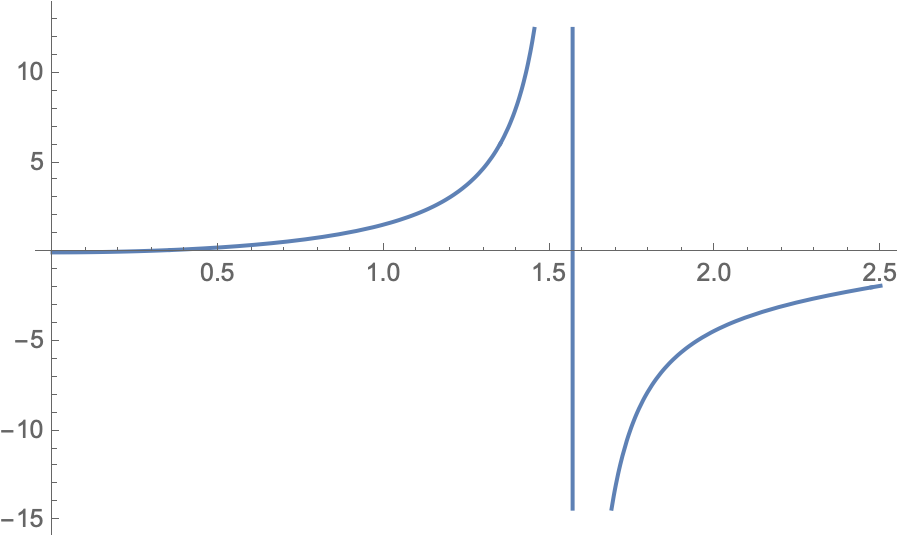
\includegraphics[scale=0.4]{xtanx.png}
                \caption{$y=x \tan{x}$}

            \end{subfigure}
              
        \end{figure}

        奇宇称涉及到的函数图像如下
        \begin{figure}[H]
            \centering
            \begin{subfigure}{0.48\textwidth}
                    
                \centering
                \wolframgraphics[png]{Plot[y=-x*Cot[x],{x,0,2.5}]}{-xcotx}
                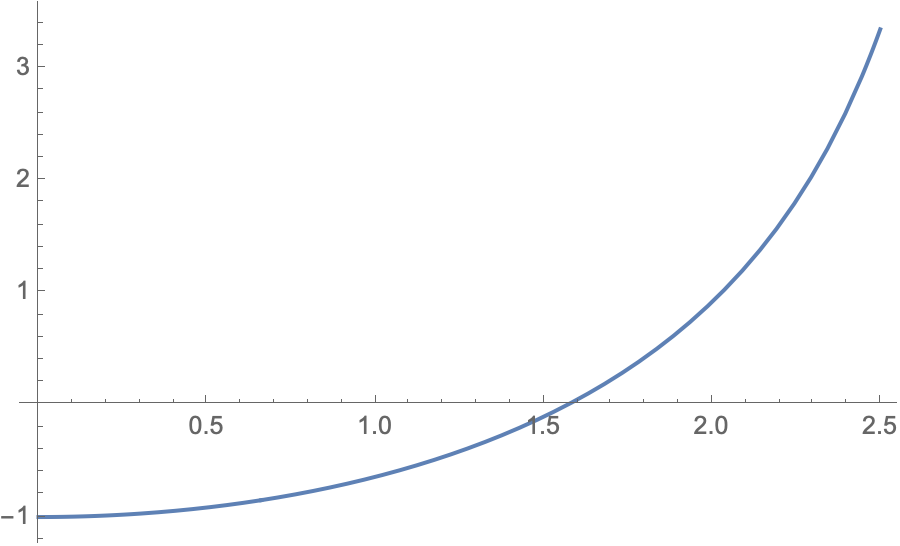
\includegraphics[scale=0.4]{-xcotx.png}
                \caption{$y=-x \cot{x}$}
                
            \end{subfigure}
            \begin{subfigure}{0.48\textwidth}
                
                \centering
                \wolframgraphics[png]{Plot[{y=-x*Cot[x],y=x*Tan[x],y=Sqrt[4-x^2]},{x,0,2.5}]}{3plot}
                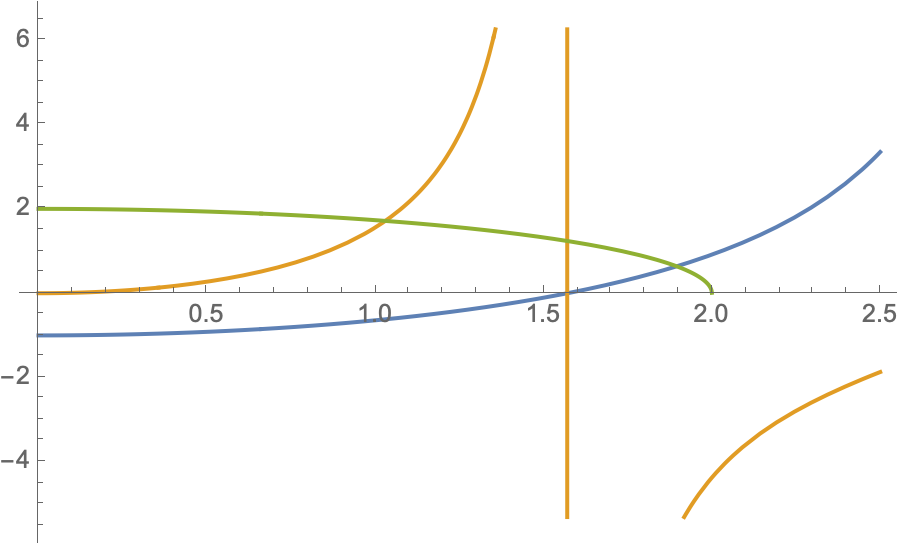
\includegraphics[scale=0.4]{3plot.png}
                \caption{三个函数曲线}

            \end{subfigure}
              
        \end{figure}

            %两个subfigure之间不能存在空行否则会出现竖排列

            
        
        由于此题的势能函数具有偶对称,因此波函数可能存在偶or奇宇称(需要分开讨论),此题中偶宇称至少存在一个交点,
        而奇宇称有解必须有条件$Q>\frac{\pi}{2}$,由题意可知存在且仅存在一个束缚态,所以保留偶宇称的唯一解即可($Q<\frac{\pi}{2}$)
        
        \subsection{一维 \texorpdfstring{$\delta$}{}势}   %使用\texorpdfstring{}{}来包括tex公式或者string需要两个参数或者仅用一个括号并用.连接
        
        先不考虑$x\neq0$的局部区域,丢掉$\delta(x)$势阱,需要用到一阶微分变化值的关系    
        
        $$ \triangle(\frac{d\psi}{dx}) = \int_{-\varepsilon}^{+\varepsilon}\frac{\hbar^2}{2\mu}V(x)\psi(x)dx $$     %\int_{}^{}   \hbar 
        
        注意不要丢了$\delta(x)$前面的参数,需要用到其积分性质
        
        $$\int_{-\varepsilon}^{+\varepsilon} \delta(x) \psi(x) dx =\psi(0) $$
        
        在归一化中,由于在$x\neq 0$其他的区域的波函数具有对称性,对其中一边积分时其值为$\frac{1}{2}$
        
        $$ \int_{0}^{+\infty}A^2 e^{-2kx} dx = \frac{1}{2} $$
        
        
    \subsection{一维分段无限深势阱}
        此题的特点是$x=0$处的$V(x)|_{x=0}=\infty$,与$\delta(x)$势不一样的是,
        虽然在此处的势能大小都是为$\infty$,但是前者的$\psi(0)=0$(也因此$\triangle \frac{d\psi}{dx}$=0,连续)而后者并不为$\psi(0)\neq0$,
        所以$\delta(x)$势通常在此点并不连续。

        当然由于$V(x)$具有偶对称性,波函数同样具有确定的宇称,现假设两个排除0点的波函数解分别为
        $$\psiii{1}{x}=B\sin(kx) \quad (0<x<a) \quad \psiii{2}{x}=D\sin(kx) \quad (-a<x<0)$$
        给两种方法通过宇称判断系数关系
        \begin{itemize}
            \item 全局判断法   \\
                若$\psi(x)$在$|x|<a$上为奇宇称,那么恰好为正弦函数$\sin(kx)$(奇函数)的形式 $\Rightarrow$ $B = D$ 
            \item 定义法    \\
                由奇宇称的定义$\psi(x)=-\psi(-x) \Rightarrow B\sin(kx)=-D\sin(-kx)=D\sin(kx) \Rightarrow B=D$ 
        \end{itemize}
        
        最后需要注意$n$的取值范围,应该是从$n=1,2,3\cdots$不能从0开始因为$ka=0 \Rightarrow k=0$(能量为0)
        
        可能在归一化中需要用到的三角函数数学公式
        $$\sin(x+y)=\sin{x} \cos{y}+\sin{y}\cos{x} \quad \cos(x+y)=\cos{x} \cos{y} - \sin{x}\sin{y}$$ 
        $$\sin(2x) = 2\sin{x} \cos{x} \quad \cos(2x) = \cos^{2}{x} - \sin^{2}{x} $$
        $$\sin^{2}{x}=\frac{1-\cos(2x)}{2} \quad \cos^{2}{x}=\frac{1+\cos(2x)}{2} $$

    \subsection{半壁无限深势阱}
        再次遇到$y=-x \cot{x}$,记忆关键点的方式可以通过极限来记忆
        $$\lim_{x \to 0}- x \cot{x} = \lim_{x \to 0} -\frac{x}{\sin{x}} + \lim_{x \to 0}\cos{x} = -1 \times 1 = -1  $$
        $$\lim_{x \to \frac{\pi}{2}}- x \cot{x} = \lim_{x \to \frac{\pi}{2}} -\frac{x}{\sin{x}} + \lim_{x \to \frac{\pi}{2}}\cos{x} = -\frac{\pi}{2} \times 0 = 0  $$
        
        最后在此题中可变参量为$a$与$V_{0}$,最好化简为不等式一边仅有可变参量,正如
        $$V_{0}a^{2}\geq \frac{\pi^{2}\hbar^{2}}{8 \mu} $$

    \subsection{复合势:\texorpdfstring{$\delta(x)$}{}和阶梯势}
        注意任何含有$\delta(x)$的势场其束缚态能量必然是负数,所以$E<0$,明确这一点再求解,同样$x=0$处波函数不连续,在求一阶微分关系时不要忘记$\delta(x)$前面的的所有系数
        此题束缚态条件比较特殊,是可解析的等式,不需要两个方程联立作图求解,最后保证一方为根式,另一方包含所有可变参量并要求$>0$即可.同时在最后的
        归一化过程中需要全空间积分为1(不是对称函数).

    \subsection{复合势:\texorpdfstring{$\delta(x)$}{}和阶梯势}
        此题直接带入波函数的连续性条件得到的方程组是难以求解的,因此需要特殊技巧
        \begin{itemize}
            \item 获得奇宇称的解,先无视$\delta(x)$势,采用无限深方势阱的解,只取在$x=\frac{a}{2}$的有效解
            \item 获得偶宇称解重点在于$\psiii{2}{a}=0$,所以不妨让$\psiii{2}{x}=A \sin{(x-a)}$,同时在$x=\frac{a}{2}$处连续得到$\psi(x)=-A \sin{(x-a)}$,它是很容易验证在关于$x=\frac{a}{2}$对称的.(设对称轴为$x=b$)
                $$\psiii{1}{b-x}=\psiii{2}{b+x} \quad \Rightarrow b=\frac{a}{2}$$
        \end{itemize}

        注意在求第一激发态的时候还没有考虑$a \to 0$,所以对于偶宇称的解的最低能量是在某一个区间,需要把两种宇称解的最低能量进行对比.

    \subsection{复合势:\texorpdfstring{$\delta(x)$}{}和谐振子势}
        加入$\delta(x)$后需要重新考虑$x=0$的一阶连续情况,也就是$\psi(0)$的值,若$\psi(0)=0$则原来的解仍成立反之不成立,所以带入$x=0$后发现是$H(0)=0$
        即可,事实上仅有$n=1,3,5\cdots$成立

    \subsection{反比例势:合流超几何函数}\label{subsec:1.8}
        关键点
        \begin{itemize}
            \item 整理微分方程形如 \quad $\frac{d^{2}\psi(x)}{d x^{2}}-k^{2}\psi(x)+\frac{\beta}{x}\psi(x)$
            \item 带入$\psi(x)=x e^{-kx}F(x)$进一步整理微分方程
            \item 变量代换$\xi \to 2kx$ 进一步整理微分方程
            \item 形如\quad $\xi \frac{d^{2}F(\xi)}{d \xi^{2}}+(\gamma-\xi)\frac{dF(\xi)}{d \xi}-\alpha F(\xi)=0$  
                  $$ E=-|E| \quad \beta=\frac{2\mu a}{\hbar^{2}} \quad \gamma=2 \quad \alpha=1-\frac{\beta}{2k}=1-\frac{\mu a}{k \hbar^{2}}$$ 
                  $$ \psi(\xi)=A\xi e^{\frac{-\xi}{2}} F(\alpha,\gamma,\xi)   $$
        \end{itemize}
        一般不考,记得反比例势能的解和合流超几何方程有关就行了,其解为合流超几何函数,此题和1.9,1.10的差不多
    
    \subsection{氢原子势能}
        见\ref{subsec:1.8}题

    \subsection{反比例势能}
        见\ref{subsec:1.8}题

    \subsection{已知波函数与\texorpdfstring{V(x)}{}的极限}\label{subsec:1.11}
        此题具有启发性,当已知波函数时,那么波函数的二阶导数同样已知,因此\sdr 方程的未知数仅有$V(x)$与$E$,可以得到$V(E,x)$方程,在利用
        额外条件进行求解,此题为$x \to +\infty \quad V \to 0$,可以解得$E$,再求解$V(x)$ 

        求导的时候需要小心,此题的二阶导一共有4项
    
    \subsection{已知波函数与\texorpdfstring{V(x)}{}的均值}
        同题目\ref{subsec:1.11}类似,不过给出另一个已知条件是$\bra{\psi}V\ket{\psi}=0$,记住利用这类已知条件时不要贸然带入波函数进行求解,应该
        凑题目条件,同时获得一个经验就是能量$E$是与坐标变量无关的,通常是优先求的,其次在得到$\int \psi^{*}E\psi dx$后不要变成$\bar{E}$,能量的平均值和
        定态能量并不是同一个东西.

    \subsection{已知能量与势能的关系}
        求解过程中注意三角函数的周期性  
        $$  \arctan{(-1)}=-\frac{\pi}{4}+n\pi \quad (n=1,2,3 \cdots ) $$    
    
    \subsection{已知两能量的本征态}
        此题的关键点
        \begin{itemize}
            \item 两个有能量的本征态具有正交性
                  $$ \int_{-\infty}^{\infty} \psiiii{1}{*}{x} \psiii{2}{x}  = 0 $$
        \end{itemize}

        但是直接利用以上正交关系来直接求得$b,c$是复杂又难以实现的,我们需要额外的关系来先求得一个参数化简第二个波函数. 

        由于$\psiii{1}{x}$的信息是完全可知的,因此我们需要利用它来获得关于$V(x)$的信息,本题可得到$V(x)$具有偶对称性,因此我们可以化简$\psiii{2}{x}$,
        只能存在一个偶宇称即$b=0$.

        这个积分可拆分成如下两个积分
            $$ \intff c e^{-\beta x^{2}} dx  \quad + \quad   \intff x^{2} e^{-\beta x^{2}} dx=0 \quad (1)$$   
        
        
        \begin{formal}
        这两个积分相当典型,在后面使用高斯试探函数经常会遇到此类积分,现总结
        

        \begin{enumerate}
            \item 
                $$ \intff e^{-a (x+b)^{2}} dx = \sqrt{\frac{\pi}{a}} $$
            \begin{proof}
                \pfindent 

                $$I=\intff e^{-a x^{2}} dx$$
                $$I^{2}= \intff e^{-a (x^{2}+y^{2})} dx dy $$

                令$x=r\cos{\theta} \quad y=r\sin{\theta}$
                $$ I^{2} = \int_{0}^{+\infty} \int_{0}^{2\pi} e^{-a r^{2}} rdrd\theta $$
               
                \begin{align*}
                    I^{2} &= \int_{0}^{+\infty} \pi  e^{-a r^{2}}d(r^{2})   \\
                          &= \frac{\pi}{a}  \lra I = \sqrt{\frac{\pi}{a}} 
                \end{align*}
            
            \end{proof}

            \item 
                $$ \intff x^{2} e^{-a x^{2}} dxdx = \frac{1}{2a} \sqrt{\frac{\pi}{a}} $$

                特别的当$n=1,3,5,7\cdots$
                $$ \intff x^{n} e^{-a x^{2}} dxdx = 0 $$

                \begin{proof}
                    \pfindent
                    $$ \frac{d(e^{-a x^{2}})}{dt} = -2a x e^{-a x^{2}} $$
                    
                    \begin{align*}
                        I &= -\frac{1}{2a} \intff x d(e^{-a x^{2}})                                         \\
                          &= -\frac{1}{2a} (\eval{x e^{-a x^{2}}}_{-\infty}^{+\infty} - \intff e^{-a x^{2}}dx )
                    \end{align*}

                    洛必达法则
                    $$ \lim_{x \to \pm \infty} x e^{-x^{2}} = \eval{\frac{1}{2x e^{x^{2}}}}_{x \to \pm \infty} = 0^{+} \quad and \quad 0^{-} $$ 
                    $$ I = \frac{1}{2a} \sqrt{\frac{\pi}{a}}$$

                \end{proof}

            \item 表格积分法(处理复杂分部积分函数):被积函数的结构为---(多项式)(函数)\quad(本质是分部积分)
                $$ \int(x^{2}+x) e^{3x} dx \quad \int x(x-a)\sin{2x} \quad \int e^{3x}\sin{2x}dx $$
                记为$f(x) \quad g(x)$

              
                \begin{center}

                    \begin{tabular}{|c|c|c|c|c|}
                        
                        \hline
                        $f(x)$ & $f'(x)$        & $f''(x)$          & $\cdots$ & 0 \\
                        \hline
                        $g(x)$ & $\int g(x) dx$ & $\iint g(x) dxdx$ & $\cdots$ & $\iiint \dots$ \\
                        \hline
                        
                    \end{tabular}
                    
                \end{center}
                
                第二行的项数与第一行保持一致,共计[n,n]

                $+(1,2)-(2,3)+(3,4)-(4,5)\cdots + c$ \quad 
                
                注意:(i,i+1)表示第一行第$i$个元素$\times$第二行的第$(i+1)$个元素,每一个乘积前的正负号为[+,-,+,...]交替,同时不要漏掉积分常数$c$,如果
                第一行的函数无法求导到0,求导直到出现原函数的常数倍也可以.($\int e^{3x}\sin{2x}dx $的积分第一行第三项为原函数的$-\frac{9}{4}$倍)
            \end{enumerate}   
        \end{formal}

        回到原积分$I_{1}+I_{2}=0$,第一个积分值很容易知道为$c \sqrt{\frac{\pi}{\beta}}$,第二个积分值为$\frac{1}{2\beta} \sqrt{\frac{\pi}{\beta}}$,求得$ c = -\frac{1}{2\beta}$

        方程(9)带入波函数求解复杂,需要细心,其中有一部需要分解因式(具有启发性,二阶导为原函数的一个多项式倍)
        \begin{align*}
            \frac{\psiiii{2}{''}{x}}{\psiii{2}{x}} & = \frac{\beta (2\beta^{2} x^{4} -11\beta x^{2} +5)}{2\beta x^{2}-1} \\
                                        & = \frac{\beta (2\beta x^{2} - 1) (\beta x^{2}-5)}{2\beta x^{2}-1}   \\
                                        & = \beta(\beta x^{2}-5) 
        \end{align*}
        
        \subsection{圆圈运动}

        此题的$x$是以圆环的外周长为度量的,需要变换波函数的变量便于求解$x=R\varphi$,因此$\frac{d}{dx^{2}}=\frac{1}{R^{2}d\varphi^{2}}$

        此时$V(x)=a\delta(x-L/2) \lra V(\varphi) = a \delta[R(\varphi-\pi)]$
        值得注意的一个$\delta(x)$的缩放性质
            $$ \intff \delta(Rx)dx = \intff \frac{1}{R} \delta(Rx) d(Rx) = 1 \lra \delta(Rx) = \frac{1}{R}\delta(x)$$

        所以我们得到新的势函数$V(\varphi) = \frac{a}{R} \delta(\varphi-\pi) $,在求解过程中不使用三角函数解,使用复幂指数的解更合适(涉及角度),\quad $\psi(x) = Ae^{-ik\varphi} + Be^{ik\varphi}$

        连续性条件发生变化,发散点为$\varphi = \pi$,实际上第三个条件和第一个条件给出的结论是一样的,而第二个条件往往是被忽略的
        $$ \psi_{1}(0) = \psi_{2}(2\pi) \quad \psi_{1}'(0) = \psi_{2}'(2\pi)\quad \psi_{1}(\pi) = \psi_{2}(\pi) $$
        
        由前两个条件可以得到如下两个方程组
        \begin{align}
            A+B&=C+D\\
            A-B&=C-D
        \end{align}

        容易解出$A=C$带入方程$(1)or(2)$会得到$B=D$,$A$与$B$的关系需要一阶波函数在$\varphi=\pi$的连续性关系解出,之后我们需要再将复幂指数的解在返回三角函数形式并
        归一化得到
        $$ \psi(x) = \sqrt{\frac{1}{\pi}} \sin{m \varphi} $$
        
        存在一个隐藏的周期性边界条件限制$m$的取值
        $$ \psi(\varphi) = \psi(\varphi+2\pi) \lra 2m\varphi = 2n\pi \quad (n=1,2,3,4\cdots) \lra m = 1,2,3,4\cdots $$
        
        由此我们可以反解出
        $$ E_{n} = \frac{\hbar^{2} m^{2}}{2\mu R^{2}} \quad (m=1,2,3,4\cdots)$$

        \subsection{改变哈密顿量求本征值(表象变换)}
            此题的关键在于表象的变换,由坐标表象转化到动量表象(详见曾书$P_{151}$和$P_{281-6}$)
            $$ \vu*{x} = i\hbar \pdv{\vu*{p}}$$

            \begin{proof}
                \pfindent

                $$ \psiii{p}{x} = \frac{1}{(2 \pi \hbar)^{\frac{n}{2}}} e^{\frac{ipx}{\hbar}} $$ 
                $$ \delta(x) = \frac{1}{(2\pi)^{n}} \intff e^{ipx} dp $$
                $$ \delta(p) = \frac{1}{(2\pi)^{n}} \intff e^{-ipx} dx $$

                n为维数,这里取1进行证明,证明前须知
                
                内积$\braket{x}{\psi}$就是波动力学的波函数
                $$\psi (x) \xlongequal{def} \braket{x}{\psi}$$
                
                进一步可知动量在坐标表象下即为动量波函数
                $$ \braket{x}{p} = \frac{1}{(2 \pi \hbar)^{\frac{n}{2}}} e^{\frac{ipx}{\hbar}} $$
                $$ \braket{p}{x} = \frac{1}{(2 \pi \hbar)^{\frac{n}{2}}} e^{\frac{-ipx}{\hbar}} $$

                算符$\vu*{x}$在坐标表象下的形式为$x$,同理算符$\vu*{p}$在动量表象下为$p$
                $${\vu*{x}} \ket{x}= x \ket{x} \quad {\vu*{p}} \ket{p} = p \ket{p} $$

                关于$\delta$函数
                $$ \braket{x'}{x} = \delta(x'-x) $$

                坐标算符在自己坐标表象下的矩阵元
                $$ x_{x'x''} = \mel{x'}{\vu*{x}}{x''} = x' \braket{x'}{x''} = x' \delta(x'-x'') $$

                \begin{align*}
                    x_{p'p''} &= \mel{p'}{x}{p''} \\
                            &= \braket{p'}{x'} \mel{x'}{x}{x''} \braket{x''}{p''}                                                                  \\
                            &= \frac{1}{(2 \pi \hbar)} \iint e^{\frac{-ip' x'}{\hbar}}  e^{\frac{ip''x''}{\hbar}} x' \delta(x'-x'') dx'dx''          \\
                            &= \frac{1}{(2 \pi \hbar)} \int x' e^{\frac{-ix(p'-p'')}{\hbar}}   dx'                                                   \\
                            &= \frac{1}{(2 \pi)} \int x' e^{-i(p'-p'')\frac{x}{\hbar}}   d(\frac{x'}{\hbar})
                \end{align*}

                积分内恰好出现了一个$x'$也就是坐标算符
                $$ \dv{e^{\frac{-ix(p'-p'')}{\hbar}}}{p'} = -\frac{i}{\hbar} e^{\frac{-ix(p'-p'')}{\hbar}}$$
                $$ e^{\frac{-ix(p'-p'')}{\hbar}} = i\hbar \dv{}{p'} e^{\frac{-ix(p'-p'')}{\hbar}}$$
                
                因此
                \begin{align*}
                     \frac{1}{(2 \pi)} \int x' e^{\frac{-ix(p'-p'')}{\hbar}}   dx' &=  \frac{1}{(2 \pi)}  i\hbar \dv{}{p'} 2\pi \delta(p'-p'')    \\
                                                                                  &= i \hbar \dv{}{p'} \delta(p'-p'')                          \\                                   
                \end{align*}

                有了矩阵元后,考虑算符的一般作用
                $$ \ket{\varphi} = \vu*{x} \ket{\psi} \lra \braket{p}{\varphi}=\mel{p}{\vu*{x}}{\psi} \lra \varphi_{p} = \int dp' x_{pp'} \psi_{p'}$$
                $$ \varphi_{p'} =  \int dp'' [x_{p'p''}] \psi_{p''} = \int dp'' [i \hbar \dv{}{p'} \delta(p'-p'')] \psi_{p''} = i\hbar \dv{}{p'} \psi_{p'} $$

                
            
            \end{proof}


        \subsection{期望值问题}
            此题涉及到两种绘景的选择:薛定谔绘景和海森堡景
            
            \begin{formal}

                \begin{itemize}
                    \item 
                    \textbf{薛定谔绘景} 

                    此绘景下,负责时间演化的算符是一种幺正算符($ UU^{*} = U^{*}U = I_{n} \quad U^{-1} = U^{*} $),态向量$\ket{\psi(0)}_{s}$,经过时t,演化到$\ket{\psi(t)}_{s}$,演化方程表示为
    
                    $$ \ket{\psi(t)}_{s} = U(t,0) \ket{\psi(0)}_{s} $$
    
                    $U(t,0)$是时间从0流易到t的时间演化算符(或者写为时间$t_{0}$),是幺正算符,假设系统哈密顿量$H$不含时间,则时间演化算符为
    
                    $$ U(t,0) = e^{\frac{-iHt}{\hbar}} $$
    
                    而且时间演化算符与哈密顿量对易,注意指数函数$e^{\frac{-iHt}{\hbar}}$必须通过泰勒级数进行计算

                    \item   
                    \textbf{海森堡绘景} 

                    态向量$\ket{\psi(t)}_{H}$,算符$A_{H}(t)$的定义分别为
                    $$ \ket{\psi(t)}_{H} \xlongequal{def} \ket{\psi(0)}_{H} = \ket{\psi(0)}_{s}$$
                    $$ A_{H}(t) \xlongequal{def} U^{\dagger}(t,0)A_{s}U(t,0) $$

                    时间演化算符对时间的偏导数为
                    $$ \pdv{U(t,0)}{t} = \frac{1}{i\hbar} H U(t,0) $$
                    $$ \pdv{U^{\dagger}(t,0)}{t} = - \frac{1}{i\hbar} U^{\dagger}(t,0) H$$

                    所以算符$A_{H}(t)$对时间的导数为
                    $$ \dv{A_{H}(t)}{t} = \frac{1}{i \hbar} [U^{\dagger} A_{s} U,U_{\dagger} H U]$$

                    不含时间的哈密顿量在两种绘景下完全一样
                    $$ H_{H} = U^{\dagger} H_{s} U = H_{s} =H $$

                    将算符的定义纳入考虑,得到海森堡运动方程
                    $$ \dv{A_{H}(t)}{t} = \frac{1}{i\hbar} [A_{H}(t),H] $$
                    $$ \dv{<A_{H}(t)>}{t} = \frac{1}{i\hbar} \overline{[A_{H}(t),H]} $$
                \end{itemize}

                宁外在解题过程中需要用到一个特殊的对易关系
                $$ [\vu*{x} , F(\vu*{p})] = i\hbar F'(\vu*{p}) \llra [\vu*{x} , \vu*{p}^{n}] = i\hbar n \vu*{p}^{n-1} $$
                


                
            \end{formal}
            

        \subsection{转子演化问题}
            自由转子和自由粒子的解的形式相似
            $$ \psi = A e^{-imx} + Be^{imx} $$
            
            通常两个传播方向会将其合并
            $$ \psi_{m} = A e^{imx} $$ 

            但是自由转子具有周期性边界条件$ \psi(x) = \psi(x+2\pi) $因此使得$m$的取值只有整数$ m = 0,\pm{1},\pm{2},\pm{3}\cdots $,也正因为是分立指标,所以
            和自由粒子有所不同,可以简单的写成求和.
            
            波函数由多个波函数线性
            组合而成
            $$ \psi(\varphi,t) = \sum_{m} c_{m} \psiii{m}{\varphi} U(t,0 ) $$

            所以题目要求我们求出处于新的能量基态概率$\abs{c_{0}}^{2}$,因此我们先要求出$c_{m}$,事实上它是由初始条件决定的(初始波函数)

            同样的在我们已知了初始波函数与初始能量,初始波函数仍然可以用$\psiii{m}{\varphi}$展开($t=0,U(0,0)=1$)
            $$ \psi(\varphi,0) = \sum_{m} c_{m} \psi_{m}(\varphi) $$
            $$ \psiiii{n}{*}{\varphi} \psi(\varphi,0) = \sum_{m} c_{m} \psiiii{n}{*}{\varphi} \psiii{m}{\varphi} $$

            对其进行积分,只留下了$c_{m}$项进行积分
            $$ \int \psiiii{m}{*}{\varphi} \psi(\varphi,0) d\varphi = \int c_{m} \psiiii{m}{*}{\varphi} \psiii{m}{\varphi} d\varphi $$
            $$ c_{m} =  \int_{0}^{\varphi_0} \psiiii{m}{*}{\varphi} \psi(\varphi,0) d\varphi$$
            
            令$m=0$
            $$ c_{0} = \int_{0}^{\varphi_0} \sin{\frac{\pi \varphi}{\varphi_{0}}} d\varphi  = \frac{2\varphi_{0}}{\pi \sqrt{\phi \varphi_{0}}} $$
            $$ \abs{c_{0}}^{2} = \frac{4 \varphi_{0}}{\pi^{3}}  $$

            时间演化算符并不影响粒子处于某个态的概率,因此当移除壁垒后概率仍旧以移除前的波函数作为初始状态(初始条件),这样将初始波函数展开(移除后的波函数可解),一些特定的系数可以求解($m\neq0$无法求解)


            
            
        
        
                         
                    
                



                
            
        
        
            

            
        
        
        
        
    
        
    
    
    

      

    \section{力学量算符}


    \section{表象}


    \section{三维定态问题}

    \section{近似方法}

    \section{自旋}

    \section{全同粒子体系}

    \section{散射}
    
    


  
\end{document}